%!TEX program = xelatex
\documentclass{article}
\usepackage{LaTeX-Submodule/template}

% Additional packages & macros
\usepackage{accsupp} % PDF accessibility options

%% Prevent user from selecting numbers when selecting code
\newcommand\emptyaccsupp[1]{\BeginAccSupp{ActualText={}}#1\EndAccSupp{}}

%% Custom prompt for listings environment
%%% https://tex.stackexchange.com/a/42056/224487

%%% Save the original way of printing the number
\let\othelstnumber=\thelstnumber
\def\customlinemarker#1#2{
    \edef\thelstnumber{%
        \unexpanded{%
            \ifnum#1=\value{lstnumber}\relax
              #2%
            \fi}%
        \ifx\thelstnumber\relax\else
        \expandafter\unexpanded\expandafter{\thelstnumber}%
        \fi
    }
}

% Header and footer
\newcommand{\unitName}{Programming Principals}
\newcommand{\unitTime}{Semester 1, 2022}
\newcommand{\unitCoordinator}{Dr Alan Woodley}
\newcommand{\documentAuthors}{\textsc{Tarang Janawalkar}}

\fancyhead[L]{\unitName}
\fancyhead[R]{\leftmark}
\fancyfoot[C]{\thepage}

% Copyright
\usepackage[
    type={CC},
    modifier={by-nc-sa},
    version={4.0},
    imagewidth={5em},
    hyphenation={raggedright}
]{doclicense}

\date{}

\begin{document}
%
\begin{titlepage}
    \vspace*{\fill}
    \begin{center}
        \LARGE{\textbf{\unitName}} \\[0.1in]
        \normalsize{\unitTime} \\[0.2in]
        \normalsize\textit{\unitCoordinator} \\[0.2in]
        \documentAuthors
    \end{center}
    \vspace*{\fill}
    \doclicenseThis
    \thispagestyle{empty}
\end{titlepage}
\newpage
%
\tableofcontents
\newpage
%
\lstset{language=[Sharp]C}
\lstset{morekeywords={with,is,as}}
\lstset{numbers=left, firstnumber=1, numberstyle=\ttfamily\emptyaccsupp}
\section{Programming}
\begin{definition}
    Programming is the process of designing and building an executable
    computer program to accomplish a specific computing result or to
    perform a specific task.
\end{definition}
Programming involves:
\begin{enumerate}
    \item Analysis
    \item Design
    \item Implementation
    \item Testing
\end{enumerate}
\subsection{Analysis}
\begin{itemize}
    \item What is the problem?
    \item What data is involved --- input, output?
    \item What is the relationship between input and output?
    \item What other constraints?
\end{itemize}
\subsection{Design}
\begin{itemize}
    \item Specify modules that need to be created to implement the solution.
    \item Module --- group of closely related functions and data they need to do their job
    \item Which parts of the problem are closely related? They probably belong together in a module.
    \item How do modules fit together and communicate?
    \item How can I test each of these modules to be sure they behave as desired?
    \item How can I test the complete system to be sure it behaves as desired?
\end{itemize}
\subsection{Implementation}
\begin{itemize}
    \item Create working software to ``do'' each part of the design
    \item Select suitable algorithms and data structures to do each required item of functionality
    \item Write code to implement the algorithms and data structures
\end{itemize}
\subsection{Testing}
\begin{itemize}
    \item Before we write any code we should have a very clear idea how the program can be validated; usually that is done by testing
\end{itemize}
\section{Types and Expressions}
\subsection{Expressions}
\begin{definition}[Expressions]
    An expression is a combination of values, variables and operators.
    In interactive mode, an interpreter evaluates expressions and displays the result.
    However, in a script, we must first compile the program to an executable in order
    to perform any tasks.
\end{definition}
\begin{definition}[Type]
    The type of an expression is ``what kind of data'' the expression carries.
\end{definition}
\begin{definition}[Variables]
    Variables are a kind of expression which have an \textbf{identity} and a \textbf{value}.

    The \textbf{value} of a variable may change as a program runs, however in
    a statically typed language, the \textbf{type} of each variable is
    specified before it can be used, and \underline{never changes}.

    Variables can be declared as follows
    \begin{lstlisting}[numbers=none]
TYPE IDENTIFIER;
TYPE IDENTIFIER = EXPRESSION;\end{lstlisting}
    In the first instance, we declare the type of the variable without initialising it.
    In the second case we declare and initialise the variable.
\end{definition}
\begin{definition}[Literal]
    The term \textit{literal} refers to the literal representation of a value.
    For example, when disambiguating between the variable \lstinline!dog!
    and the string \lstinline!"dog"! we would say the \emph{``variable dog''} % chktex 18
    vs.\ the \emph{``string literal dog''}.
\end{definition}
C\# identifiers must take the following into account
\begin{itemize}
    \item Identifiers can contain letters, digits and the underscore character (\lstinline!_!)
    \item Identifiers must begin with a letter
    \item Identifiers cannot contain whitespaces
    \item Identifiers are case sensitive (``\lstinline!Foo!'' and ``\lstinline!foo!'' are different variables) % chktex 38
    \item Reserved words such as C\# keywords cannot be used as identifiers
\end{itemize}
\subsection{Types}
There are 9 integer and 3 floating-point types in C\#, each with a different size and range. The minimum and maximum
values of any type can be determined using \lstinline!TYPE.MinValue! and \linebreak \lstinline!TYPE.MaxValue!.
\begin{table}[H]
    \centering
    \begin{tabular}{c c c}
        \toprule
        \textbf{C\# type}  & \textbf{Size} & \textbf{Range}                \\
        \midrule
        \lstinline!sbyte!  & 8 bit         & \(-2^7\) to \(2^7 - 1\)       \\
        \lstinline!byte!   & 8 bit         & \(0\) to \(2^8 - 1\)          \\
        \lstinline!short!  & 16 bit        & \(-2^{15}\) to \(2^{15} - 1\) \\
        \lstinline!ushort! & 16 bit        & \(0\) to \(2^{16} - 1\)       \\
        \lstinline!int!    & 32 bit        & \(-2^{31}\) to \(2^{31} - 1\) \\
        \lstinline!uint!   & 32 bit        & \(0\) to \(2^{32} - 1\)       \\
        \lstinline!long!   & 64 bit        & \(-2^{63}\) to \(2^{63} - 1\) \\
        \lstinline!ulong!  & 64 bit        & \(0\) to \(2^{64} - 1\)       \\
        \bottomrule
    \end{tabular}
    \caption{Integer types in C\#.}
    % \label{}
\end{table}
\begin{table}[H]
    \centering
    \begin{tabular}{c c c c}
        \toprule
        \textbf{C\# type}   & \textbf{Size} & \textbf{Range}                                              & \textbf{Precision}   \\
        \midrule
        \lstinline!float!   & 32 bit        & \(\pm 1.5 \times 10^{-45}\) to \(\pm 3.4 \times 10^{38}\)   & \sim 6 to 9 digits   \\
        \lstinline!double!  & 64 bit        & \(\pm 5.0 \times 10^{-324}\) to \(\pm 1.7 \times 10^{308}\) & \sim 15 to 17 digits \\
        \lstinline!decimal! & 128 bit       & \(\pm 1.0 \times 10^{-28}\) to \(7.9228 \times 10^{28}\)    & \sim 28 to 29 digits \\
        \bottomrule
    \end{tabular}
    \caption{Floating-point types in C\#.}
    % \label{}
\end{table}
\subsection{Type Conversion}
By default, C\# automatically assigns the \lstinline!int!, \lstinline!uint!,
\lstinline!long!, or \lstinline!ulong! type to any integer depending the size and sign
of the provided number. Any floating-point number is instantiated as a \lstinline!double!.
\begingroup
\let\thelstnumber\relax
\customlinemarker{1}{\$}
\customlinemarker{3}{\$}
\customlinemarker{5}{\$}
\customlinemarker{7}{\$}
\begin{lstlisting}
(100).GetType()
[System.Int32]
(4294967295).GetType()    
[System.UInt32]
(-4294967295).GetType()
[System.Int64]
(100.0).GetType()
[System.Double]
\end{lstlisting}
\endgroup
To override this behaviour we can add a suffix to the number.
\begin{table}[H]
    \centering
    \begin{tabular}{c c}
        \toprule
        \textbf{Type}       & \textbf{Suffix}                                \\
        \midrule
        \lstinline!uint!    & \lstinline!u!                                  \\
        \lstinline!long!    & \lstinline!l!                                  \\
        \lstinline!ulong!   & \lstinline!u!, \lstinline!l! or \lstinline!ul! \\
        \midrule
        \lstinline!float!   & \lstinline!f!                                  \\
        \lstinline!double!  & \lstinline!d!                                  \\
        \lstinline!decimal! & \lstinline!m!                                  \\
        \bottomrule
    \end{tabular}
    \caption{Type suffixes for numeric types.}
    % \label{}
\end{table}
If a literal is prefixed with \lstinline!u!, its type is the first
of the following types in which its value can be represented:
\lstinline!uint!, \lstinline!ulong!.

Similarly, if a literal is prefixed with \lstinline!l!, its type is the first
of the following types in which its value can be represented:
\lstinline!long!, \lstinline!ulong!.

If the value of an integer is within the range of the destination type,
the value can be implicitly converted to the remaining integer types.
\subsubsection{Implicit Conversion}
Implicit conversions do not require any special syntax as the conversion
always succeeds and no data is lost.
The following diagram illustrates implicit conversions for numeric types.
The direction of the arrows indicate possible implicit conversions where
intermediate types can be skipped.
Note that all integer types can be converted to floating-point types.
\begin{figure}[H]
    \centering
    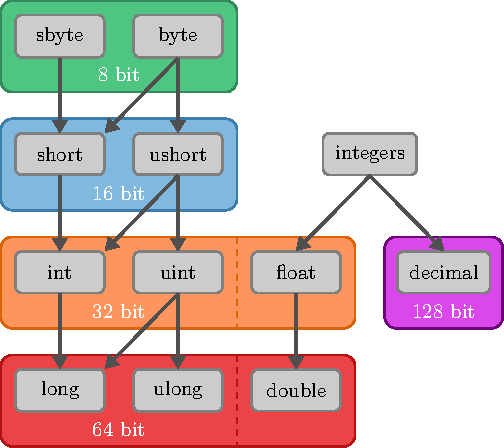
\includegraphics[height = 8cm, keepaspectratio = true]{figures/implicit_conversions.pdf}
    \caption{Numeric type implicit conversions in C\#.}
    % \label{}
\end{figure}
For example
\begingroup
\let\thelstnumber\relax
\customlinemarker{1}{\$}
\customlinemarker{2}{\$}
\customlinemarker{4}{\$}
\customlinemarker{7}{\$}
\customlinemarker{8}{\$}
\customlinemarker{10}{\$}
\begin{lstlisting}
// 8 bit unsigned integer to 64 bit signed integer 
byte b = 32; Console.WriteLine($"{b} {b.GetType()}")
32 System.Byte
long l = b; Console.WriteLine($"{l} {l.GetType()}")
32 System.Int64

// 16 bit signed integer to double precision floating-point number
short s = 30000; Console.WriteLine($"{s} {s.GetType()}")
30000 System.Int16
double d = s; Console.WriteLine($"{d} {d.GetType()}")
30000 System.Double
\end{lstlisting}
\endgroup
\subsubsection{Explicit Conversion}
When a conversion cannot be made without risking losing information,
the compiler requires that we perform an explicit conversion using a \textbf{type cast}.
The syntax for a type cast is as follows
\begin{lstlisting}[numbers=none]
(NEW_TYPE) EXPRESSION
\end{lstlisting}
For example
\begingroup
\let\thelstnumber\relax
\customlinemarker{1}{\$}
\customlinemarker{2}{\$}
\customlinemarker{4}{\$}
\customlinemarker{7}{\$}
\customlinemarker{8}{\$}
\customlinemarker{10}{\$}
\begin{lstlisting}
// Decimal to single precision floating-point number
decimal pi = 3.14159265358979323m; Console.WriteLine($"{pi} {pi.GetType()}")
3.14159265358979323 System.Decimal
float fPi = (float) pi; Console.WriteLine($"{fPi} {fPi.GetType()}")
3.141593 System.Single

// 32 bit unsigned integer to 8 bit signed integer
uint u = 9876; Console.WriteLine($"{u} {u.GetType()}")
9876 System.UInt32
byte b = (byte) u; Console.WriteLine($"{b} {b.GetType()}")
148 System.Byte
\end{lstlisting}
\endgroup
In the final example, to understand what is happening in the explicit conversion,
we must look at the binary representation of the two integers.
\begingroup
\let\thelstnumber\relax
\customlinemarker{1}{\$}
\customlinemarker{3}{\$}
\begin{lstlisting}
uint u = 9876; Console.WriteLine(Convert.ToString(u, 2).PadLeft(32, '0'))
00000000000000000010011010010100
byte b = (byte) u; Console.WriteLine(Convert.ToString(b, 2).PadLeft(8, '0'))
10010100
\end{lstlisting}
\endgroup
Notice that the value is determined by copying the 8 least significant bits
from the 32 bit unsigned integer.
\subsection{Operators}
The following table lists the C\# operators starting with the highest precedence to the lowest.
\begin{table}[H]
    \centering
    \begin{tabular}{>{\centering}p{0.45\linewidth} c}
        \toprule
        \textbf{Operators}                                                                                           & \textbf{Category}                 \\
        \midrule
        \lstinline!x.y!, \lstinline!f(x)!, \lstinline!a[i]!, \lstinline!x++!,
        \lstinline!x--!, \lstinline?x!?, \lstinline!x->y! and other keywords                                         & Primary                           \\
        \lstinline!+x!, \lstinline!-x!, \lstinline+!x+, \lstinline!~x!,
        \lstinline!++x!, \lstinline!--x!, \lstinline!^x!, \lstinline!(T)x!, \lstinline!await!,
        \lstinline!&x!, \lstinline!*x!, \lstinline!true!, \lstinline!false!                                          & Unary                             \\
        \lstinline!x..y!                                                                                             & Range                             \\
        \lstinline!switch!, \lstinline!with!                                                                         & ---                               \\
        \lstinline!x * y!, \lstinline!x / y!, \lstinline!x % y!                                                      & Multiplicative                    \\
        \lstinline!x + y!, \lstinline!x - y!                                                                         & Additive                          \\ % chktex 8
        \lstinline!x << y!, \lstinline!x >> y!                                                                       & Shift                             \\
        \lstinline!x < y!, \lstinline!x > y!, \lstinline!x <= y!, \lstinline!x >= y!, \lstinline!is!, \lstinline!as! & Relational and type-testing       \\
        \lstinline!x == y!, \lstinline?x != y?                                                                       & Equality                          \\ % chktex 26
        \lstinline!x & y!                                                                                            & Logical {\ttfamily{AND}}          \\
        \lstinline!x ^ y!                                                                                            & Logical {\ttfamily{XOR}}          \\
        \lstinline!x | y!                                                                                            & Logical {\ttfamily{OR}}           \\
        \lstinline!x && y!                                                                                           & Conditional {\ttfamily{AND}}      \\
        \lstinline!x || y!                                                                                           & Conditional {\ttfamily{OR}}       \\
        \lstinline!x ?? y!                                                                                           & Null-coalescing operator          \\ % chktex 26
        \lstinline!c ? t : f!                                                                                        & Conditional operator              \\ % chktex 26
        \lstinline!x = y!, \lstinline!=>! and shorthand assignments                                                  & Assignment and lambda declaration \\
        \bottomrule
    \end{tabular}
    \caption{Precedence of various operators in C\#.}
    % \label{}
\end{table}
In C\#, arithmetic operations behave as expected.
\begingroup
\let\thelstnumber\relax
\customlinemarker{1}{\$}
\customlinemarker{3}{\$}
\customlinemarker{5}{\$}
\customlinemarker{7}{\$}
\customlinemarker{9}{\$}
\begin{lstlisting}
123 + 12
135
123 - 12
111
123 * 12
1476
123 / 12
10
123 % 12
3
\end{lstlisting}
\endgroup
Binary operators always convert the resulting data type to the data type of the
argument with the largest size in memory
(with a few exceptions when converting between floating-point types).
Each result in the above examples have the type \lstinline!System.Int32!.

Hence division between two 32 bit integers truncates any floating-point precision.
\begingroup
\let\thelstnumber\relax
\customlinemarker{1}{\$}
\customlinemarker{3}{\$}
\customlinemarker{5}{\$}
\customlinemarker{7}{\$}
\begin{lstlisting}
123 / 12
10
123.0 / 12
10.25
123 / 12.0
10.25
123.0 / 12.0
10.25
\end{lstlisting}
\endgroup
Here the final three results are converted to the type \lstinline!System.Double!
using the reasoning given above.
\subsection{Characters}
A character type represents a \textbf{single} Unicode UTF-16 character.
Character objects can be implicitly converted to 16 bit unsigned integers and
support the comparison, equality, increment and \linebreak decrement operators.

A character is initialised using single quotation marks (\lstinline!'!). % chktex 38
\begingroup
\let\thelstnumber\relax
\customlinemarker{1}{\$}
\customlinemarker{3}{\$}
\customlinemarker{5}{\$}
\customlinemarker{7}{\$}
\customlinemarker{9}{\$}
\begin{lstlisting}
char c = 'A'; c
'A'
c.GetType()
[System.Char]
c++
'B'
(ushort) c
69
c == 69
true
\end{lstlisting}
\endgroup
\subsection{Strings}
A string is a sequential read-only collection of character objects.
A string is initialised using double quotation marks (\lstinline!"!). % chktex 18
\begingroup
\let\thelstnumber\relax
\customlinemarker{1}{\$}
\customlinemarker{3}{\$}
\begin{lstlisting}
string s = "Hello, World!"; s
"Hello, World!"
s.GetType()
[System.String]
\end{lstlisting}
\endgroup
\subsubsection{String Indexing}
The characters in a string can be accessed by position (starting at 0).
\begingroup
\let\thelstnumber\relax
\customlinemarker{1}{\$}
\customlinemarker{3}{\$}
\begin{lstlisting}
s[0]
'H'
s[s.Length - 1]
'!'
\end{lstlisting}
\endgroup
\subsubsection{Immutability}
In C\#, string objects are immutable meaning that the string cannot be modified in memory. If a new string is assigned
to this object, it will simply point to a new location in memory.
\begingroup
\let\thelstnumber\relax
\customlinemarker{1}{\$}
\customlinemarker{3}{\$}
\customlinemarker{6}{\$}
\begin{lstlisting}
string s = "String with tyop."; s
"String with tyop."
s[14] = 'p';
(1,1): error CS0200: Property or indexer 'string.this[int]' cannot be assigned 
to -- it is read only
s = "String without typo."
"String without typo."
\end{lstlisting}
\endgroup
\subsubsection{Escape Sequences}
To use special characters such as newlines, tabs, backslashes, or double quotation marks, we must
use an escape sequence.
\begingroup
\let\thelstnumber\relax
\customlinemarker{1}{\$}
\begin{lstlisting}
string s = "This is a quotation mark \".\nThis line appears on a new line."; s
"This is a quotation mark \".\nThis line appears on a new line."
\end{lstlisting}
\endgroup
Note that the string is evaluated as a string literal. To view this string verbatim, we must use
\lstinline!Console.WriteLine!.
\begingroup
\let\thelstnumber\relax
\customlinemarker{1}{\$}
\begin{lstlisting}
Console.WriteLine(s) 
This is a quotation mark ".
This line appears on a new line.
\end{lstlisting}
\endgroup
\subsubsection{Verbatim String Literals}
If a string contains many escape sequences we can use verbatim strings for convenience.
\begingroup
\let\thelstnumber\relax
\customlinemarker{1}{\$}
\customlinemarker{3}{\$}
\begin{lstlisting}
string s = @"String with multiple escape sequences ""This is a quote"".
This line appears on a new line.";
Console.WriteLine(s)
String with multiple escape sequences "This is a quote".
This line appears on a new line.
\end{lstlisting}
\endgroup
\subsubsection{Format Strings}
To dynamically determine a string at runtime, we can use format strings.
There are two methods to create format strings: string interpolation and composite formatting.

String interpolation allows us to reference variable names directly inside a string.
Interpolated strings are identified by the dollar sign.
\begingroup
\let\thelstnumber\relax
\customlinemarker{1}{\$}
\customlinemarker{2}{\$}
\begin{lstlisting}
int a = 40; int b = 13;
$"Given a = {a} and b = {b}, a + b = {a + b}"
"Given a = 40 and b = 13, a + b = 53"
\end{lstlisting}
\endgroup
Composite formatting uses placeholders for variables which must be provided in order of reference.
Here the same variable can be referenced many times in a string.
\begingroup
\let\thelstnumber\relax
\customlinemarker{1}{\$}
\customlinemarker{2}{\$}
\customlinemarker{4}{\$}
\customlinemarker{6}{\$}
\begin{lstlisting}
int a = 40; int b = 13;
string.Format("Given a = {0} and b = {1}, a + b = {2}", a, b, a + b)
"Given a = 40 and b = 13, a + b = 53"
string.Format("a + b = {2} where a = {0} and b = {1}", a, b, a + b)
"a + b = 53 where a = 40 and b = 13"
string.Format("We can reference `a` twice, here {0} and here {0}", a)
"We can reference `a` twice, here 40 and here 40"
\end{lstlisting}
\endgroup
\subsubsection{Numeric to String Conversion}
Strings can be concatenated with numeric variables
\begingroup
\let\thelstnumber\relax
\customlinemarker{1}{\$}
\customlinemarker{2}{\$}
\begin{lstlisting}
int a = 25;
"The temperature is " + a + " degrees."
"The temperature is 25 degrees."
\end{lstlisting}
\endgroup
As the \lstinline!+! operator is evaluated from left to right, the following string concatenation
will not evaluate the sum of 1, 2, and 3.
\begingroup
\let\thelstnumber\relax
\customlinemarker{1}{\$}
\begin{lstlisting}
"sum = " + 1 + 2 + 3
"sum = 123"
\end{lstlisting}
\endgroup
The \lstinline!ToString()! method can be accessed from all numeric types, with a
format specifier which indicates the number of precision to display.
\begingroup
\let\thelstnumber\relax
\customlinemarker{1}{\$}
\customlinemarker{3}{\$}
\customlinemarker{5}{\$}
\begin{lstlisting}
(1498).ToString("G3")
"1.5E+03"
(1498).ToString("F3")
"1498.000"
(1498).ToString("C2")
"$1,498.00"
\end{lstlisting}
\endgroup
These format specifiers can be applied directly in interpolated strings.
\begingroup
\let\thelstnumber\relax
\customlinemarker{1}{\$}
\customlinemarker{2}{\$}
\begin{lstlisting}
int i = 1498;
$"{i:G3}, {i:F3}, {i:C2}"
"1.5E+03, 1498.000, $1,498.00"
\end{lstlisting}
\endgroup
We can also add specify padding in interpolated strings.
\begingroup
\let\thelstnumber\relax
\customlinemarker{1}{\$}
\customlinemarker{2}{\$}
\begin{lstlisting}
decimal pi = 3.14159265358979323m;
$"Pi with left padding {pi, 10:F6}"
"Pi with left padding   3.141593"
\end{lstlisting}
\endgroup
For more information see: \href{https://docs.microsoft.com/en-us/dotnet/standard/base-types/custom-numeric-format-strings}{\textit{Custom numeric format strings}}.
\subsubsection{String to Numeric Conversion}
We can convert a string to a number by calling the \lstinline!Parse! method found on numeric types,
or by using methods in the \lstinline!System.Convert! class.
\begingroup
\let\thelstnumber\relax
\customlinemarker{1}{\$}
\customlinemarker{3}{\$}
\begin{lstlisting}
double.Parse("2.718281")
2.718281
Convert.ToDouble("2.718281")
2.718281
\end{lstlisting}
\endgroup
\section{Structured Programming}
Structured programming relies on three constructs: sequence, selection and iteration.
These help us control the flow of our programs.
\subsection{Sequence}
\subsubsection{Blocks}
In C\# we can group statements together inside a scope by using braces \lstinline!{ }!.
The statements inside this block are executed in order as a single instruction.
\begingroup
\let\thelstnumber\relax
\customlinemarker{1}{\$}
\customlinemarker{2}{.}
\customlinemarker{3}{.}
\customlinemarker{4}{.}
\customlinemarker{5}{.}
\customlinemarker{7}{\$}
\begin{lstlisting}
int i = 5;
{
    i = 10;
    Console.WriteLine(i);
}
10
Console.WriteLine(i);
10
\end{lstlisting}
\endgroup
Here \lstinline!i! is accessed as an enclosing locally scoped variable.
\emph{This behaviour is akin to blocks defined in selection and iteration structures.}
\subsubsection{Nested Blocks}
Here is another example that utilises nested blocks and demonstrates access.
\begingroup
\let\thelstnumber\relax
\customlinemarker{1}{\$}
\customlinemarker{2}{\$}
\customlinemarker{3}{.}
\customlinemarker{4}{.}
\customlinemarker{5}{.}
\customlinemarker{6}{.}
\customlinemarker{7}{.}
\customlinemarker{8}{.}
\customlinemarker{9}{.}
\customlinemarker{10}{.}
\customlinemarker{11}{.}
\customlinemarker{12}{.}
\customlinemarker{13}{\$}
\begin{lstlisting}
// Global scope    
{
    // Block 1     
    int i = 5;  
    Console.WriteLine(i);
    {
        // Block 2
        i += 5;
        Console.WriteLine(i);
    }
    // i = 10
}
Console.WriteLine(i);
5
10
(1,19): error CS0103: The name 'i' does not exist in the current context
\end{lstlisting}
\endgroup
In this example we see that the variable \lstinline!i! is local to block 1 and therefore accessible to block 2.

However, the converse is not true. \lstinline!i! cannot be accessed by its enclosing scope
as local variables are destroyed when a block ends.

We also cannot declare a variable in a block that shares its name
with another variable in its enclosing local scope.
\begingroup
\let\thelstnumber\relax
\customlinemarker{1}{\$}
\customlinemarker{2}{.}
\customlinemarker{3}{.}
\customlinemarker{4}{.}
\customlinemarker{5}{.}
\customlinemarker{6}{.}
\begin{lstlisting}
{
    int i = 5;
    {
        int i = 5;
    }   
}
(4,13): error CS0136: A local or parameter named 'i' cannot be declared
in this scope because that name is used in an enclosing local scope to 
define a local or parameter
\end{lstlisting}
\endgroup
\subsection{Selection}
Selection allows us to choose from a range of different options.
\subsubsection{If Statements}
If statements have the following syntax.
\begin{lstlisting}[numbers=none]
// Single statement
if (CONDITION) STATEMENT;
// Multiple statements
if (CONDITION)
{
    STATEMENTS
}
\end{lstlisting}
In both cases, \lstinline!CONDITION! is an expression that returns a Boolean value % chktex 13
when evaluated. If this value is \lstinline!true!, the subsequent statement(s) will
be executed. Conversely, if the expression yields \lstinline!false!, the subsequent
statement(s) will be ignored and control passes to the next statement after the \lstinline!if!
statement.
\subsubsection{If-else Statements}
We can add an alternative statement if \lstinline!CONDITION! is \lstinline!false! using an \lstinline{else} % chktex 13
clause.
\begin{lstlisting}[numbers=none]
// Single statement
if (CONDITION) STATEMENT_1 else STATEMENT_2;
// Multiple statements
if (CONDITION) 
{
    STATEMENTS_1
} else
{
    STATEMENTS_2;
}
\end{lstlisting}
This structure differs to the previous example slightly as either \lstinline!STATEMENT_1! or \lstinline!STATEMENT_2!
will be executed. Again the decision depends on the Boolean value returned by the condition.
\subsubsection{Nested if Statements}
The blocks in an \lstinline!if! statement can also allow us to nest any number of
\lstinline!if! statements to create a more complex flow of control.
\begin{lstlisting}[numbers=none]
if (CONDITION_1) if (CONDITION_2) STATEMENT_2 else STATEMENT_1;
// Written using braces
if (CONDITION_1) 
{
    if (CONDITION_2) 
    {
        STATEMENT_2
    }
} else 
{
    STATEMENT_1
}
\end{lstlisting}
Generally nested \lstinline!if! statements are difficult to read and should be avoided if possible.
\subsubsection{Cascading if Statements}
An alternative to nested \lstinline!if! statements are cascading \lstinline!if! statements.
These statements allow us to provide controlled alternatives to an \lstinline!if-else! statement if the
first condition returns \lstinline!false!.
\begin{lstlisting}[numbers=none]
if (CONDITION_1) 
{
    STATEMENTS_1
} else if (CONDITION_2)
{
    STATEMENTS_2
} else if (CONDITION_3)
{
    STATEMENTS_3
} 
...
else {
    STATEMENTS_N
}
\end{lstlisting}
In this structure, any statement \(1<i<n\) will be executed if
and only if all conditions before \(i\) yield \lstinline!false! and
\lstinline!CONDITION_I! yields \lstinline!true!. % chktex 13

The final statement \(n\) after the \lstinline!else! clause is executed
if all preceding conditions return \lstinline!false!.

Note that the \lstinline!else! clause may be omitted.
\subsubsection{Switch Statements}
A \lstinline!switch! statement is an alternative to cascading \lstinline!if!
statements and are another kind of multi-way branch.
\begin{lstlisting}[numbers=none]
switch (EXPRESSION) 
{
    case CONSTANT_1:
        STATEMENTS_1;
        break;
    case CONSTANT_2:
        STATEMENTS_2;
        break;
    ...
    default:
        STATEMENTS_N;
        break;
}
\end{lstlisting}
In this structure, \lstinline!EXPRESSION! is any numeric or string expression, % chktex 13
and \lstinline!CONSTANT! is a literal of matching type. % chktex 13
This means that \lstinline!STATEMENTS_I! is executed if \lstinline!EXPRESSION == CONSTANT_I!. % chktex 13

The default branch behaves similarly to an \lstinline!else! clause and is executed if all
none of the cases are satisfied.

Each branch must end with one of the following keywords depending on where the
switch statement is defined: \lstinline!break!, \lstinline!return!,
\lstinline!goto!, \lstinline!throw!, or \lstinline!continue!.
\subsection{Iteration}
Iterative constructs allow us to repeat statements zero, one, or many times,
without making multiple copies of the statement.
\subsubsection{While Statements}
\begin{lstlisting}[numbers=none]
while (CONDITION) 
{
    STATEMENTS
}
\end{lstlisting}
Fundamental semantics:
\begin{enumerate}
    \item Execute \lstinline!STATEMENTS! if \lstinline!CONDITION == true!. % chktex 13
    \item Goto Step 1.
\end{enumerate}
\subsubsection{Do-while Statements}
\begin{lstlisting}[numbers=none]
do 
{
    STATEMENTS
}
while (CONDITION) 
\end{lstlisting}
Fundamental semantics:
\begin{enumerate}
    \item Execute \lstinline!STATEMENTS!. % chktex 13
    \item Goto Step 1 if \lstinline!CONDITION == true!.
\end{enumerate}
\subsubsection{For Statements}
\begin{lstlisting}[numbers=none]
for (INIT; CONDITION; UPDATE) 
{
    STATEMENTS
}
\end{lstlisting}
Fundamental semantics:
\begin{enumerate}
    \item Execute \lstinline!INIT!. % chktex 13
    \item Execute \lstinline!STATEMENTS! if \lstinline!CONDITION == true!. % chktex 13
    \item Execute \lstinline!UPDATE!.
    \item Goto Step 2.
\end{enumerate}
Generally a \lstinline!while! statement is used when the number of iterations is unknown and
\lstinline!for! statements are used otherwise. Both of these structures can execute
statements either zero, one or many times.

While uncommon, \lstinline!do-while! statements are used if we want to execute
the loop body at least once.
\subsection{Jump Statements}
The following statements unconditionally transfer control:
\begin{itemize}
    \item \lstinline!break! terminates the closest enclosing iteration or switch statement
    \item \lstinline!continue! starts a new iteration of the closest enclosing iteration statement
\end{itemize}
Note that jump statements can be placed anywhere inside the loop body and that any succeeding
statements or the \lstinline!UPDATE! statement (in the \lstinline!for! structure) % chktex 13
will not be executed.
\subsection{Booleans}
A Boolean (\lstinline!bool!) is a type that has two values,
\lstinline!true! and \lstinline!false!.
Boolean expressions are expressions that when evaluated, yield a Boolean value.
\subsubsection{Comparison Operators}
Comparison operators are a common Boolean expression:
\begin{itemize}
    \item \lstinline!x == y!
    \item \lstinline+x != y+ % chktex 26
    \item \lstinline!x < y!
    \item \lstinline!x > y!
    \item \lstinline!x <= y!
    \item \lstinline!x >= y!
\end{itemize}
\subsubsection{Logical Operators}
Logical operators are also Boolean expressions:
\begin{itemize}
    \item \lstinline+!a+ (not)
    \item \lstinline!a && b! (and)
    \item \lstinline!a || b! (or)
\end{itemize}
In C\#, logical operators use short-circuit evaluation, meaning that
if the left-expression guarantees the resulting Boolean value,
the right-expression is not evaluated.

For example
\begingroup
\let\thelstnumber\relax
\customlinemarker{1}{\$}
\customlinemarker{2}{.}
\customlinemarker{3}{.}
\customlinemarker{4}{.}
\customlinemarker{5}{.}
\customlinemarker{6}{\$}
\customlinemarker{7}{.}
\customlinemarker{8}{.}
\customlinemarker{9}{.}
\customlinemarker{10}{.}
\customlinemarker{11}{\$}
\begin{lstlisting}
bool a() 
{ 
    Console.WriteLine("a was executed."); 
    return false;
}
bool b() 
{ 
    Console.WriteLine("b was executed."); 
    return true;
}
a() && b()
a was executed.
False
\end{lstlisting}
\endgroup
Here we see that the second function \lstinline!b()! was not executed
as the {\ttfamily AND} operator requires both expressions to be true,
so regardless of the value of \lstinline!b()!, the result will be
\lstinline!false!.

Similarly for {\ttfamily OR}:
\begingroup
\let\thelstnumber\relax
\customlinemarker{1}{\$}
\customlinemarker{2}{.}
\customlinemarker{3}{.}
\customlinemarker{4}{.}
\customlinemarker{5}{.}
\customlinemarker{6}{\$}
\customlinemarker{7}{.}
\customlinemarker{8}{.}
\customlinemarker{9}{.}
\customlinemarker{10}{.}
\customlinemarker{11}{\$}
\begin{lstlisting}
bool a() 
{ 
    Console.WriteLine("a was executed."); 
    return false;
}
bool b() 
{ 
    Console.WriteLine("b was executed."); 
    return true;
}
b() || a()
b was executed.
True
\end{lstlisting}
\endgroup
Here only one of the two expressions need to be \lstinline!true!
for the result to be true. However, if we reversed the order of
the expressions:
\begingroup
\let\thelstnumber\relax
\customlinemarker{1}{\$}
\customlinemarker{2}{.}
\customlinemarker{3}{.}
\customlinemarker{4}{.}
\customlinemarker{5}{.}
\customlinemarker{6}{\$}
\customlinemarker{7}{.}
\customlinemarker{8}{.}
\customlinemarker{9}{.}
\customlinemarker{10}{.}
\customlinemarker{11}{\$}
\begin{lstlisting}
bool a() 
{ 
    Console.WriteLine("a was executed."); 
    return false;
}
bool b() 
{ 
    Console.WriteLine("b was executed."); 
    return true;
}
a() || b()
a was executed.
b was executed.
True
\end{lstlisting}
\endgroup
we can see that since \lstinline!a()! does not guarantee
the resulting value, we must also evaluate \lstinline!b()!.

The {\ttfamily NOT} operator simply negates the value of the Boolean expression.
\section{Collections}
\subsection{Arrays}
If we want to effectively manage groups of related objects, we can utilise arrays and collections.
When defining an array of type \lstinline!T!, we must append the type with square brackets \lstinline![ ]!.
\begin{lstlisting}[numbers=none]
TYPE[] IDENTIFIER;
TYPE[] IDENTIFIER = EXPRESSION;
\end{lstlisting}
As a result, each item must have the same data type. To specify the array size, we can initialise
the variable with the \lstinline!new! expression.
\begin{lstlisting}[numbers=none]
TYPE[] IDENTIFIER = new TYPE[SIZE];
// Alternatively
TYPE[] IDENTIFIER;
IDENTIFIER = new TYPE[SIZE];
\end{lstlisting}
\subsection{Access}
To access the array, we can use the identifier for that array. Each object within
an array can be distinguished by its subscript (or index). To access the object within
an array, we place the index inside square brackets \lstinline![i]! and append this to the 
identifier. 
\begingroup
\let\thelstnumber\relax
\customlinemarker{1}{\$}
\customlinemarker{2}{\$}
\customlinemarker{4}{\$}
\customlinemarker{6}{\$}
\customlinemarker{8}{\$}
\customlinemarker{10}{\$}
\begin{lstlisting}
int[] intArray = new int[3]; 
intArray
int[3] { 0, 0, 0 }
intArray[0] = 1; intArray[0]
1
intArray[1] = 2; intArray[0]
2
intArray[2] = 3; intArray[0]
3
intArray
int[3] { 1, 2, 3 }
\end{lstlisting}
\endgroup
Note that array indexing starts at 0. If the value of the elements inside the array
are known when the array is initialised, we can set the element values using the following syntax.
\begin{lstlisting}[numbers=none]
TYPE[] IDENTIFIER = new TYPE[SIZE] { element1, element2, ..., elementN };
TYPE[] IDENTIFIER = new TYPE[] { element1, element2, ..., elementN };
TYPE[] IDENTIFIER = { element1, element2, ..., elementN };
\end{lstlisting}
Note that when using the first method, the number of elements \(N\) must be equal to the specified \lstinline!SIZE!. % chktex 13
\subsection{Array Representation in Memory}
To be able to access an array by index, the elements must be stored contiguously in memory, that is,
stored one after the other. This means that each element \(i\) is \(i \times S_T\) bytes from \(i = 0\), 
where \(S_T\) is the size of the array type.
\subsection{Default Values}
If an array is declared without initialisation, then each element takes one of the following
default values based on the type:
\begin{description}
    \item[Numeric] \lstinline!0!
    \item[Character] \lstinline!\u0000! or \lstinline!null!
    \item[Boolean] \lstinline!false!
\end{description}
\subsection{ForEach Loops}
The \lstinline!foreach! statement provides a simple, clean way to iterate through the elements of an array,
without using the element index.
\begingroup
\let\thelstnumber\relax
\customlinemarker{1}{\$}
\customlinemarker{2}{\$}
\customlinemarker{3}{.}
\customlinemarker{4}{.}
\customlinemarker{5}{.}
\begin{lstlisting}
int[] array = { 1, 2, 3 };
foreach (int i in array)
{
    Console.WriteLine(i);
}
1
2
3    
\end{lstlisting}
\endgroup
Note that the values \lstinline!i! are readonly, and hence this structure 
does not modify the elements of an array.

If we wanted to modify these values, can we use either a \lstinline!while! or
\lstinline!for! loop. The following example increments each value of an array 
using a \lstinline!for! loop.
\begingroup
\let\thelstnumber\relax
\customlinemarker{1}{\$}
\customlinemarker{2}{\$}
\customlinemarker{3}{.}
\customlinemarker{4}{.}
\customlinemarker{5}{.}
\customlinemarker{6}{\$}
\begin{lstlisting}
int[] array = { 1, 2, 3 };
for (int i = 0; i < array.Length; i++)
{
    array[i]++;
}
array
int[3] { 2, 3, 4 }
\end{lstlisting}
\endgroup
\subsection{Compound Arrays}
When we have two or more arrays of values that share
the same indices, we can implement compound arrays to 
create a correspondence between those arrays.
\subsubsection{Parallel Arrays}
Parallel arrays are useful when the various arrays
hold different types of data. In this method, multiple 
single dimensional arrays are created.
\begingroup
\let\thelstnumber\relax
\customlinemarker{1}{\$}
\customlinemarker{2}{\$}
\customlinemarker{3}{\$}
\customlinemarker{4}{.}
\customlinemarker{5}{.}
\customlinemarker{6}{.}
\begin{lstlisting}
string[] item = { "Shoes", "Shirt", "Pants" };
int[] price = { 100, 40, 80 };
for (int i = 0; i < item.Length; i++) 
{
    Console.WriteLine($"Item: {item[i]}\tPrice: {price[i]:C}");
}
Item: Shoes     Price: $100.00
Item: Shirt     Price: $40.00
Item: Pants     Price: $80.00
\end{lstlisting}
\endgroup
Although there are benefits to using this approach, larger data
sets with multiple columns may be better represented in a 
multidimensional array.
\subsubsection{Multidimensional Arrays}
Multidimensional arrays behave similarly to regular arrays
but use different declaration and access syntax. 
\begin{lstlisting}[numbers=none]
// 2D arrays
TYPE[,] IDENTIFIER = new TYPE[SIZEX, SIZEY];
// nD arrays
TYPE[,,...] IDENTIFIER = new TYPE[SIZEX, SIZEY, ...];
\end{lstlisting}
When declaring the type, it is important to specify the correct
number of commas (\lstinline!,!). The number of commas is equal to 
the number of dimensions minus 1.

When instantiating the array on the right hand side of the assignment,
the length of each dimension is specified as an integer, and is separated by a comma.
Similar to single dimensional arrays, we can set the values when we declare the array.
\begingroup
\let\thelstnumber\relax
\customlinemarker{1}{\$}
\customlinemarker{2}{.}
\customlinemarker{3}{\$}
\begin{lstlisting}
int[,] array2d = {{ 2, 3 },
                  { 1, 5 }};
array2d
int[2, 2] { { 2, 3 }, { 1, 5 } }
\end{lstlisting}
\endgroup
Multidimensional arrays are commonly separated at each dimension
so that they are easier to read. 

When accessing the value from a multidimensional array, 
we must separate each index using a comma.
\begingroup
\let\thelstnumber\relax
\customlinemarker{1}{\$}
\customlinemarker{2}{\$}
\customlinemarker{4}{\$}
\customlinemarker{5}{.}
\customlinemarker{6}{.}
\customlinemarker{7}{.}
\customlinemarker{8}{.}
\customlinemarker{9}{.}
\customlinemarker{10}{.}
\begin{lstlisting}
int ROW = array2d.GetLength(0);
int COL = array2d.GetLength(1);

for (int i = 0; i < ROW; i++)
{
    for (int j = 0; j < COL; j++)
    {
        Console.WriteLine($"The value at ({i}, {j}) is {array2d[i, j]}");
    }
}
The value at (0, 0) is 2
The value at (0, 1) is 3
The value at (1, 0) is 1
The value at (1, 1) is 5
\end{lstlisting}
\endgroup
Here the \lstinline!GetLength()! methods are used to find the length 
of both the first and second dimensions.
\subsection{Lists}
Lists allow us to have variable size arrays, meaning we can 
add and remove elements during execution.
\begin{lstlisting}[numbers=none]
List<TYPE> IDENTIFIER = new List<TYPE>();
List<TYPE> IDENTIFIER = new List<TYPE>{ elements };
\end{lstlisting}
Initially the first technique creates a list with 0 elements, 
also known as its \textit{count}.
We can add to this list using the \lstinline!Add()! method, and
remove from it using the \lstinline!Remove()! method.
\begingroup
\let\thelstnumber\relax
\customlinemarker{1}{\$}
\customlinemarker{2}{\$}
\customlinemarker{4}{\$}
\customlinemarker{5}{\$}
\customlinemarker{6}{\$}
\customlinemarker{7}{\$}
\customlinemarker{8}{\$}
\customlinemarker{9}{\$}
\customlinemarker{10}{\$}
\begin{lstlisting}
List<int> list = new List<int>();
list
List<int>(0) { }
list.Add(3)
list.Add(1)
list.Add(4)
list.Add(5)
list.Add(1)
list.Add(5)
list
List<int>(6) { 3, 1, 4, 5, 1, 5 }
\end{lstlisting}
\endgroup
By using the \lstinline!Remove()! method, we can remove the 
accidental 5 that appears at index 3.
\begingroup
\let\thelstnumber\relax
\customlinemarker{1}{\$}
\customlinemarker{3}{\$}
\customlinemarker{5}{\$}
\customlinemarker{7}{\$}
\begin{lstlisting}
list.Remove(5)
true
list
List<int>(5) { 3, 1, 4, 1, 5 }
list.Remove(7)
false
list
List<int>(5) { 3, 1, 4, 1, 5 }
\end{lstlisting}
\endgroup
From the first \lstinline!Remove()!, 
only the first \lstinline!5! was removed from the list.
The method also returned a Boolean value indicating that the value 
\lstinline!5! existed in the list. When we try to remove the 
number \lstinline!7!, the method returns \lstinline!false!,
as the list does not contain a \lstinline!7!, and hence the 
list remains unchanged.
\section{Methods}
\subsection{Programming Complexity}
Programming logic is usually complex as it involves modelling rules
and constraints from the real world. 

When dealing with complexity, we must guarantee:
\begin{itemize}
    \item Correctness
    \begin{itemize}
        \item Software must be trustworthy
        \item Software must meet requirements
        \item Valid inputs must always produce the required outcomes
    \end{itemize}
    \item Robustness
    \begin{itemize}
        \item Programs should not crash
    \end{itemize}
    \item Efficiency
    \begin{itemize}
        \item Programs must complete their work in a timely manner
        \item Programs should utilise efficient algorithms
        \item Programs should avoid unnecessary loops and convoluted logic, 
        i.e., using existing standard libraries rather than writing our own code
    \end{itemize}
\end{itemize}
We can use methods to address this complexity be decomposing large tasks into smaller tasks.
\begin{itemize}
    \item Each sub-task handles part of the larger problem
    \item Each sub-task can be implemented separately as a method or group of methods
    \item Tests can be developed to target each method individually
\end{itemize}
As long as each sub-task is correct, robust, and efficient, the overall program will be also.
As sub-tasks are simpler than the original problem, these goals are easier to achieve.

Methods can also help eliminate duplicate code, so that code is more compact, and by
moving them into libraries, we can use them in other projects making programming
more productive.
\subsection{Declaring Methods}
A method has the following syntax
\begin{lstlisting}[numbers=none]
[ACCESS_MODIFIER] RETURN_TYPE METHOD_IDENTIFIER(PARAMETER_LIST)
{
    STATEMENTS
}    
\end{lstlisting}
\subsubsection{Access Modifiers}
Access modifiers will be discussed in a later section.
\subsubsection{Return Types}
A return type specifies what type of value is returned to the method caller.
If a method alters the state of the program and does not
necessarily require an output, is a side effect method and its return type is  
\lstinline!void!.
\subsubsection{Identifiers}
The identifier is the name of the method, which can be any valid C\# identifier.
By convention, method identifiers are camel case with an upper-case first letter.
\subsubsection{Parameter List}
The parameter list declares the formal parameters of the method, i.e., 
what arguments may be passed to the method. The parameter list is 
a comma separated list of parameters that have the following syntax
\begin{lstlisting}[numbers=none]
[PARAMETER_MODIFIER] TYPE PARAMETER_IDENTIFIER [= DEFAULT_VALUE]
\end{lstlisting}
The parameter modifier tells the compiler whether to send an argument by reference
or by value. There are 4 modifiers to choose from
\begin{itemize}
    \item \lstinline!in! --- Arguments are passed by reference but cannot be modified.
    \item \lstinline!ref! --- Arguments are passed by reference and can be modified.
    \item \lstinline!out! --- Arguments are passed by reference but must be initialised inside the method.
    \item \lstinline!params! --- A variable number of arguments are passed by value.
\end{itemize}
By default, if a modifier is not specified, the argument is generally passed by value.

The parameter type specifies what type of argument is to be passed. The parameter identifier 
gives the argument an alias within the method's scope, and 
default values can be assigned to parameters if they are optional.

Note that parameters do not need to be re-declared inside the method.
\subsubsection{Statements}
The statements inside a method can consist of sequences of statements
including declarations, expressions, and structured blocks.
As a method introduces a nested block, all variables declared in a method body
are local to the method.
\subsection{Invoking Methods}
To call a method we can invoke it using the following syntax
\begin{lstlisting}[numbers=none]
METHOD_IDENTIFIER(ARGUMENT_LIST)
\end{lstlisting}
If a method is defined in another class, we must qualify the name 
with the appropriate class:
\begin{lstlisting}[numbers=none]
CLASS_NAME.METHOD_IDENTIFIER(ARGUMENT_LIST)
\end{lstlisting}
\subsubsection{Argument List}
The argument list can be empty or a list of comma-separated expressions, 
corresponding to the formal parameter list in the same order encountered.
\begin{lstlisting}[numbers=none]
[PARAMETER_MODIFIER] EXPRESSION
\end{lstlisting}
If the corresponding formal parameter is \lstinline!ref! or \lstinline!out!,
the argument must also be qualified with the corresponding modifier.

If we do not want to provide arguments in order, or if certain 
optional parameters wish to be skipped, we can do so by
providing the name of the parameter identifier using the following syntax.
\begin{lstlisting}[numbers=none]
PARAMETER_IDENTIFIER: [PARAMETER_MODIFIER] EXPRESSION
\end{lstlisting}
This allows us to provide arguments in an arbitrary order.
\subsubsection{Control Return}
When control is returned to the method caller, the method
may provide an output if its return type is non-void.
In this event, the method call can be treated as an expression
and it can be assigned to a variable.
\begin{lstlisting}[numbers=none]
RETURN_TYPE IDENTIFIER = METHOD_IDENTIFIER(ARGUMENT_LIST)
\end{lstlisting}
Here the identifier being assigned the output must have the same
type as the return type of the method.
\subsection{Argument Types}
While we can use parameter modifiers to force value type variables to be 
sent by reference, certain structure types are implicitly passed by reference.

Objects such as arrays are a pointer to a location in memory so that
instead of passing a copy of that array into the method, 
the address of its location is passed. 

This allows the array elements to be modified from within 
the method.
\end{document}
